% Статья о платформе «Кадровый ассистент».
% Сборка: python build_figures.py && tectonic kadry-paper.tex (из папки docs/paper) -> kadry-paper.pdf.
\documentclass[10pt,a4paper,twocolumn]{article}

\usepackage[a4paper,top=2.1cm,bottom=2.3cm,left=1.9cm,right=1.9cm,columnsep=0.68cm]{geometry}
\usepackage{fontspec}
\usepackage[russian]{babel}
\setmainfont{LibertinusSerif}[Extension=.otf,UprightFont=*-Regular,BoldFont=*-Bold,
  ItalicFont=*-Italic,BoldItalicFont=*-BoldItalic]
\setsansfont{LibertinusSans}[Extension=.otf,UprightFont=*-Regular,BoldFont=*-Bold,
  ItalicFont=*-Italic]
\setmonofont{DejaVuSansMono}[Extension=.ttf,Scale=0.80,BoldFont=*-Bold]

\usepackage{graphicx}
\usepackage{booktabs}
\usepackage{tabularx}
\usepackage{array}
\usepackage{enumitem}
\usepackage{caption}
\usepackage{amsmath}
\usepackage[round]{natbib}
\usepackage{xcolor}
\usepackage[colorlinks=true,linkcolor=blue!50!black,citecolor=blue!50!black,
  urlcolor=blue!50!black]{hyperref}
\usepackage{tikz}
\usetikzlibrary{positioning,arrows.meta,fit,calc}

\setlist{nosep,leftmargin=1.2em}
\captionsetup{font=small,labelsep=colon}
\setlength{\parskip}{0pt}
\setlength{\textfloatsep}{10pt plus 2pt minus 2pt}
\setlength{\dbltextfloatsep}{11pt plus 2pt minus 2pt}
\emergencystretch=1.8em
\renewcommand{\bibname}{Литература}
\renewcommand{\refname}{Литература}
\newcommand{\code}[1]{\texttt{#1}}
\newcommand{\dotg}{\textcolor{green!55!black}{$\bullet$}}
\newcommand{\doty}{\textcolor{orange!85!black}{$\bullet$}}
\newcommand{\dotr}{\textcolor{red!70!black}{$\bullet$}}
\newcommand{\dotw}{\textcolor{black!45}{$\circ$}}
\newcolumntype{L}{>{\raggedright\arraybackslash}X}

\tikzset{
  box/.style={draw=black!70,rounded corners=2pt,fill=blue!4,align=center,
    font=\footnotesize,inner sep=3.5pt,minimum height=0.82cm},
  core/.style={box,fill=orange!10},
  store/.style={box,fill=green!7},
  guard/.style={box,fill=red!6},
  arr/.style={-{Stealth[length=1.9mm]},black!70},
  lbl/.style={font=\scriptsize,text=black!70,align=center},
}

\title{\bfseries Кадровый ассистент: платформа подбора, оценки\\
  и сопровождения муниципальных служащих,\\
  где LLM извлекает факты, а решает код}
\author{%
  \textbf{Родион Музыкант, Анастасия Безусова, Илья Бурмистров,}\\
  \textbf{Мария Ворона, Денис Чичеров, Давид Егиазарян}\\[2pt]
  Команда №\,9 (GORKY) · НИУ ВШЭ — Нижний Новгород\\[2pt]
  \small\url{https://github.com/team-gorky-9/hr}\quad·\quad\url{https://gorky.bond}}
\date{}

\begin{document}
\maketitle

\begin{abstract}
Подбор и сопровождение муниципальных служащих регулируются жёстче коммерческого найма:
требования закреплены в должностных инструкциях и нормативных актах (25-ФЗ, 99-З), персональные
данные защищены 152-ФЗ, а кадровые решения вправе принимать только уполномоченный сотрудник.
Прямое применение языковых моделей («загрузить резюме и получить процент пригодности») в таких
условиях неприменимо: модель склонна к галлюцинациям, не различает отсутствие сведений и
отрицание опыта, а произвольный балл нельзя проверить по источнику. В статье описана
реализованная архитектура платформы «Кадровый ассистент» (коммит \code{c87cbd6}): девять
FastAPI-сервисов за Nginx-шлюзом с изоляцией персональных данных до вызова LLM и строгим
разделением ответственности — языковая модель извлекает структурированные факты с цитатами, а
верификацию цитат (с координатами UTF-16), арифметику пересекающихся интервалов стажа $[L, U]$,
применимость публикации, светофор ранжирования, поиск по опыту, иммутабельную отчётность с
моделью полноты и расчёт независимого покрытия по алгоритму Куна выполняет детерминированный код.
На реальном архиве из 1\,739 файлов (287 DOCX-откликов папки «консультант») показано, что 7,3\,\%
документов относятся к другим должностям и ещё 15,7\,\% не имеют подвала публикации; на живом
прогоне YandexGPT (41 кейс формальных правил, \code{assessment-2.0.2}) достигнуто 41/41 при 0
ошибок модели; на контрольном бенчмарке поиска BM25 превосходит плотный E5 по скорости в 6,4 раза
(4,33 против 27,50\,мс) и точности выдачи при нуле ложных срабатываний.
\end{abstract}

\section{Введение}

Кадровая служба администрации крупного города одновременно обрабатывает сотни разнородных
откликов (HH.ru, «Работа России», сайт администрации, обращения по 59-ФЗ, студенческая практика),
контролирует обратную связь от отраслевых департаментов, оформляет комплекты документов, ведёт
адаптацию и готовит управленческую отчётность. На практике возникают три системные проблемы,
подтверждённые аудитом реального архива организаторов (\code{kadry-2026}, 1\,739 файлов):
\begin{enumerate}
  \item \textbf{Неоднородность и шум на входе.} Даже внутри одной архивной папки резюме
    приходят без единого шаблона, содержат «Историю общения» площадки и смешивают отклики на
    разные должности.
  \item \textbf{Недопустимость «чёрного ящика».} В муниципальной службе нельзя отказать
    кандидату на основании «совпадения 64\,\%» от нейросети: каждое требование должно иметь
    проверяемое основание в тексте, а нехватка сведений в резюме — вести к уточняющему вопросу,
    а не к скрытому отсеву.
  \item \textbf{Потеря контекста и недостоверность цифр.} После передачи резюме в департамент
    обратная связь теряется, а в сводных отчётах отсутствие данных из источника часто
    отображается как ноль.
\end{enumerate}

Платформа «Кадровый ассистент» решает эти задачи за счёт пяти архитектурных принципов,
реализованных в действующем коде (\code{c87cbd6}):
\begin{itemize}
  \item \textbf{Изоляция ПДн до вызова LLM:} контакты и ФИО выносятся в отдельную таблицу
    \code{candidate\_pii} на этапе импорта; языковая модель получает только очищенный текст,
    а каждый просмотр контактов кадровиком фиксируется в \code{audit\_log}.
  \item \textbf{Детерминированный допуск до LLM:} версионный реестр публикаций
    (\code{app/postings/}) проверяет соответствие отклика должности и утверждённому профилю
    до запуска модели.
  \item \textbf{Проверяемая опора на цитаты и код вместо баллов:} LLM извлекает факты и цитаты,
    а верификацию подстрок, понижение неподтверждённых выводов, интервальную арифметику стажа
    $[L, U]$, скоупированные отрицания и светофор ранжирования выполняет код
    (\code{app/assessment/}).
  \item \textbf{Доказательный выбор поиска:} лексический BM25 и плотный E5 (pgvector) сравнены
    на одном контрольном наборе; по итогам замера в продакшене по умолчанию включён BM25, а
    векторная ветка вынесена под флаг конфигурации.
  \item \textbf{Честная математика отчётности и планирования:} контент-адресуемые SHA-256
    снимки строго различают подтверждённый ноль (\code{0 complete}) и отсутствие покрытия
    (\code{null unavailable}), а независимое покрытие кадровых потребностей считается алгоритмом
    максимального паросочетания Куна.
\end{itemize}

\section{Архитектура платформы}

\begin{figure*}[t]
\centering
\resizebox{\textwidth}{!}{%
\begin{tikzpicture}[node distance=0.50cm and 0.65cm]
  \node[box] (ui) {React 18 + TS SPA\\{\scriptsize 4 роли: Портал, HR,}\\{\scriptsize ОПК, Сотрудник}};
  \node[guard,right=0.85cm of ui] (gw) {Nginx 1.28 Gateway\\{\scriptsize \code{access\_log off}, 21\,MiB,}\\{\scriptsize префиксы \code{/<service>/}}};

  \node[core,right=1.0cm of gw,yshift=1.35cm] (leg) {Legacy Core (\code{app/})\\{\scriptsize ingest, postings, assessment,}\\{\scriptsize interview, search, reporting}};
  \node[box,right=1.0cm of gw,yshift=0.0cm] (pgsvc) {Workforce · Hiring · Req.\\{\scriptsize кадры, адаптация, ИПР,}\\{\scriptsize оформление, профили}};
  \node[box,right=1.0cm of gw,yshift=-1.35cm] (sqsvc) {5 сервисов жизненного цикла\\{\scriptsize students, mobility, support,}\\{\scriptsize recognition, feedback}};

  \node[box,above=0.45cm of leg] (llm) {YandexGPT API\\{\scriptsize только очищенный текст,}\\{\scriptsize без \code{candidate\_pii}}};
  \node[store,right=0.95cm of leg] (pg1) {PostgreSQL 17 + pgvector\\{\scriptsize 4 изолированные БД:}\\{\scriptsize legacy, workforce, req, hiring}};
  \node[box,right=0.95cm of pgsvc] (rmq) {RabbitMQ 4.1.8\\{\scriptsize + \code{workforce-worker}}};
  \node[store,right=0.95cm of sqsvc] (sqdb) {Изолированные тома\\{\scriptsize 5 SQLite БД + файлы}\\{\scriptsize + SHA-256 снимки отчётов}};

  \draw[arr] (ui) -- node[lbl,above]{HTTPS} (gw);
  \draw[arr] (gw.east) -- ++(0.35,0) |- (leg.west);
  \draw[arr] (gw.east) -- (pgsvc.west);
  \draw[arr] (gw.east) -- ++(0.35,0) |- (sqsvc.west);

  \draw[arr] ([xshift=-4pt]leg.north) -- node[lbl,left]{текст} ([xshift=-4pt]llm.south);
  \draw[arr] ([xshift=4pt]llm.south) -- node[lbl,right]{JSON} ([xshift=4pt]leg.north);

  \draw[arr] (leg.east) -- (pg1.west);
  \draw[arr] (pgsvc.east) -- ++(0.35,0) |- ([yshift=-6pt]pg1.west);
  \draw[arr] (pgsvc.east) -- (rmq.west);
  \draw[arr] (sqsvc.east) -- (sqdb.west);
\end{tikzpicture}}
\caption{Развёрнутая архитектура платформы «Кадровый ассистент» (\code{deploy/compose.yaml}, \code{c87cbd6}).
Девять FastAPI-сервисов работают от непривилегированного UID\,10001 с \code{cap\_drop: [ALL]} за единым
шлюзом Nginx. Персональные данные изолированы в \code{candidate\_pii} и не передаются в LLM.}
\label{fig:arch}
\end{figure*}

Система развёрнута как контейнерный стек (\code{deploy/compose.yaml}, рис.~\ref{fig:arch}):
клиентское приложение на React~18, TypeScript и Tailwind CSS взаимодействует через обратный
прокси Nginx~1.28 (\code{deploy/nginx.conf}) с девятью Python~3.13/FastAPI-сервисами
(табл.~\ref{tab:services}).

\begin{table}[t]
\centering\small
\begin{tabularx}{\columnwidth}{@{}lLl@{}}
\toprule
Контур & Функции & БД / Вход \\
\midrule
\code{legacy} & Импорт, оценка, интервью, поиск, workflow, отчёт & PG17+vec / \code{X-User} \\
\code{workforce} & Кадры, адаптация, ИПР, RabbitMQ worker & PG17 / Bearer WF \\
\code{requirements} & Профили ДИ, согласование, каталог & PG17 / Bearer WF \\
\code{hiring} & Кабинет кандидата, оформление дел & PG17 / Bearer WF \\
\code{students} & Практика, заявки, задания, итоги & SQLite / Bearer WF \\
\code{social-support} & Материальная помощь, выписки & SQLite / fixture \\
\code{feedback} & Анонимные опросы, обращения & SQLite / demo \\
\code{mobility} & Временные задачи, переходы & SQLite / fixture \\
\code{recognition} & Благодарности, события, сессии & SQLite / demo \\
\bottomrule
\end{tabularx}
\caption{Девять сервисов платформы в \code{deploy/compose.yaml}. Четыре контура используют
единый PostgreSQL~17 (изолированные роли без \code{superuser}), пять — отдельные SQLite-тома.
В UI на стенде не подключены \code{mobility} и \code{recognition} (доступны через OpenAPI).}
\label{tab:services}
\end{table}

\textbf{Эксплуатация и безопасность.} Все контейнеры запускаются от \code{UID 10001} с
\code{no-new-privileges} и \code{cap\_drop: [ALL]}; миграции выполняются одноразовыми
контейнерами до старта API. В Nginx отключён \code{access\_log}, чтобы URL с одноразовыми
кодами опросов и идентификаторами приватных документов не попадали в системные журналы, а
внутренние заголовки шлюза (\code{X-Interaction-Gateway-Key}, \code{X-Interaction-User-Id})
принудительно очищаются от клиентского трафика. Данные разделены на контуры \code{working} и
\code{training}; рабочий поиск и рабочие годовые отчёты закрыты отдельными серверными токенами.
Доставка образов автоматизирована в GitHub Actions (сборка по \code{uv.lock}, публикация в GHCR,
резервное копирование \code{backup.sh} и сквозная проверка \code{smoke.py} всех девяти OpenAPI).

\section{Импорт, защита ПДн и применимость публикаций}

\subsection{Очистка текста и изоляция ПДн (152-ФЗ)}

Модуль \code{app/ingest/} принимает пакеты \code{.txt} (UTF-32/UTF-16/UTF-8-sig/CP1251),
\code{.docx} (разбор XML без дублирования объединённых ячеек и с ограничением
\code{MAX\_DOCX\_XML = 128\,MiB} против ZIP/DTD-бомб) и текстовые \code{.pdf} через
\code{pypdf}. Сканы без текстового слоя получают код \code{PDF\_NEEDS\_REVIEW} и переводятся
в карантин без потери файла. Дедупликация выполняется по SHA-256 байтов оригинала, а
вспомогательный \code{\_TextIndex} выявляет разные файлы с совпадающим текстом.

Очистка (\code{ingest-rules v2}, \code{app/ingest/redact.py}) комбинирует регулярные правила
и морфологический классификатор имён на базе \code{pymorphy3} \citep{korobov2015morphological}.
Извлечённые ФИО, телефоны, e-mail и дата/пол из шапки HH.ru переносятся в отдельную таблицу
\code{candidate\_pii}, а в \code{candidate\_texts} сохраняется версионированный обезличенный
текст. Если после очистки остаются признаки ПДн или менее 50 значащих символов, документ уходит
в карантин. Независимый модуль \code{app.ingest.audit} повторно проверяет очищенные тексты
широкими паттернами и сверкой против значений \code{candidate\_pii}.

В языковую модель никогда не передаются ни \code{candidate\_pii}, ни сырой текст документа.
На уровне API (\code{app/api/routes.py}) контакты и ФИО отдаются только ролям \code{HR} и
\code{ADMIN} с обязательной записью \code{AuditAction.VIEW\_PII} в \code{audit\_log} и
заголовком \code{Cache-Control: private, no-store}; руководитель подразделения
(\code{department}) и анонимный доступ остаются обезличенными. На реальном архиве
\code{kadry-2026} (1\,739 файлов) конвейер импортировал 1\,721 резюме и отделил 18 служебных
документов (\code{docs/modules/ingest.md}).

\subsection{Эмпирическое обоснование реестра публикаций}

Парсер \code{app/ingest/history.py} выделяет из подвала «Истории общения» HH.ru название
публикации, на которую реально откликнулся кандидат, и внешние отклики в других конкурсах.
Проверка реальной папки «консультант» (\code{kadry-2026}, 287 DOCX-файлов, отчёт
\code{requirements-03-posting-mapping.json}, рис.~\ref{fig:postings}) выявила критический факт:
в одной кадровой папке смешаны восемь категорий документов.

\begin{figure}[t]
\centering
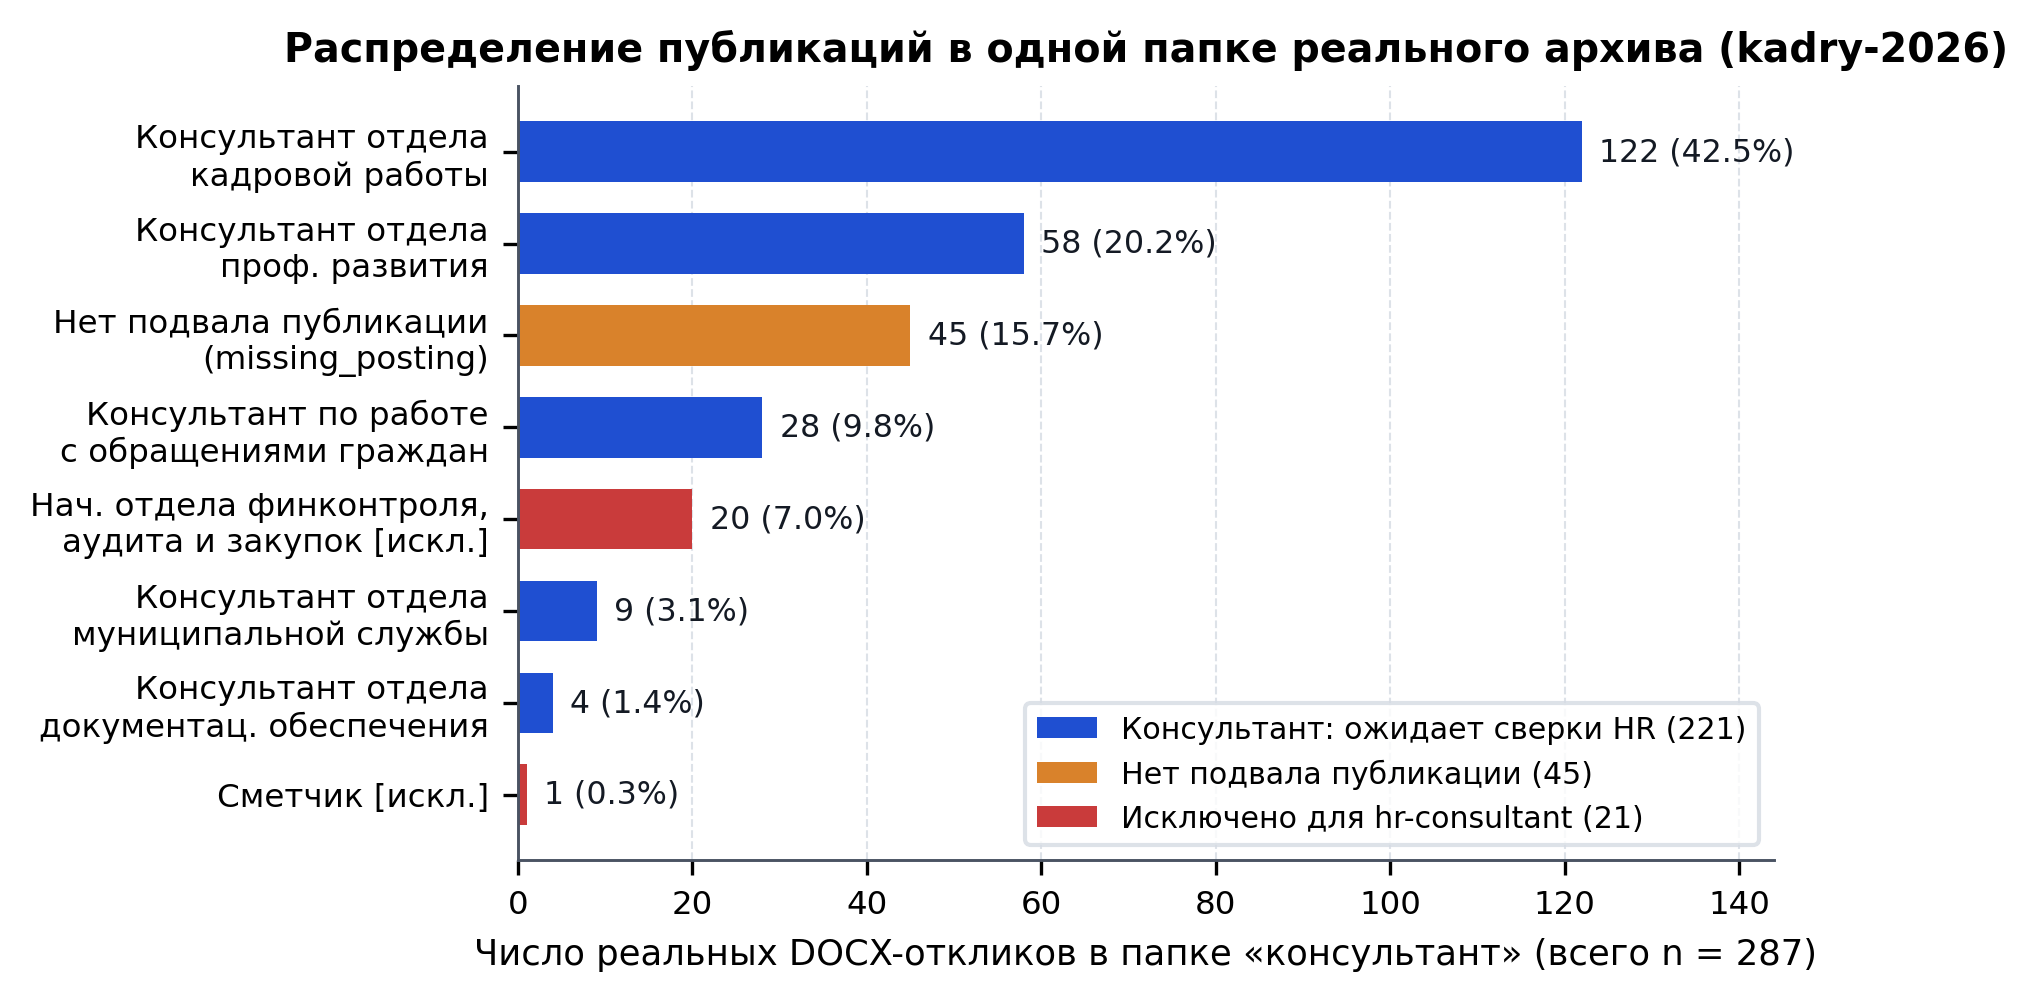
\includegraphics[width=\columnwidth]{figures/posting_distribution.png}
\caption{Фактическое распределение публикаций внутри одной папки «консультант» реального
архива \code{kadry-2026} ($n = 287$ DOCX, \code{requirements-03-posting-mapping.json}).
7,3\,\% файлов относятся к другим должностям, 15,7\,\% не имеют подвала публикации.}
\label{fig:postings}
\end{figure}

Наивный скрининг всей папки по профилю \code{hr-consultant} ошибочно оценил бы по чужим
требованиям 21 человека (7,3\,\%: 20 откликов на начальника отдела финансового контроля и 1
сметчика) и без основания обработал бы 45 файлов (15,7\,\%) без подвала публикации. Поэтому в
\code{app/postings/} реализован детерминированный реестр публикаций (\code{v2}), который по
5-компонентному контексту (\code{dataset\_id}, \code{dataset\_sha256}, \code{channel},
\code{source\_folder}, \code{is\_synthetic}) и точному названию публикации вычисляет статус
\code{confirmed}, \code{needs\_review} или \code{no\_matching\_position} до вызова LLM и при
неподтверждённой связи блокирует оценку. Аналогично профили требований
(\code{fixtures/requirement\_profiles/all\_six/}: 6 должностей, 12 формальных условий, 36
компетенций, 256 индикаторов) загружаются строго в статусе \code{draft} и допускаются к оценке
только после явного утверждения уполномоченным кадровиком.

\section{Оценка кандидатов с верификацией цитат и гайд интервью}

\subsection{Разделение ролей между LLM и кодом}

\begin{figure*}[t]
\centering
\resizebox{\textwidth}{!}{%
\begin{tikzpicture}[node distance=0.45cm and 0.55cm]
  \node[box] (txt) {Очищенный текст\\{\scriptsize \code{CandidateText} (без ПДн)}};
  \node[guard,right=0.6cm of txt] (post) {Реестр публикаций\\{\scriptsize \code{posting\_resolution} +}\\{\scriptsize утверждённый профиль}};
  \node[core,right=0.6cm of post] (llm) {LLM (YandexGPT)\\{\scriptsize \code{card-v2}, \code{assess-v4}:}\\{\scriptsize факты, периоды, цитаты}};
  \node[guard,right=0.6cm of llm] (ver) {Верификатор цитат\\{\scriptsize \code{resolve\_quote}, UTF-16,}\\{\scriptsize нет цитаты $\Rightarrow$ \code{unknown}}};
  \node[core,right=0.6cm of ver] (calc) {Детерминированный расчёт\\{\scriptsize стаж $[L,U]$, скоуп-отрицания,}\\{\scriptsize \code{same\_as}, светофор}};
  \node[box,right=0.6cm of calc] (out) {Карточка и интервью\\{\scriptsize 4 группы (\dotg\,\doty\,\dotr\,\dotw),}\\{\scriptsize \code{guide-v2} по пробелам}};

  \draw[arr] (txt) -- (post);
  \draw[arr] (post) -- (llm);
  \draw[arr] (llm) -- (ver);
  \draw[arr] (ver) -- (calc);
  \draw[arr] (calc) -- (out);
\end{tikzpicture}}
\caption{Пайплайн оценки и подготовки телефонного интервью (\code{assessment-2.0.4},
\code{guide-v2}). Языковая модель не выносит финальных вердиктов и не рассчитывает числовых
процентов: все проверки существования цитат, стажа и ранжирования выполняются кодом.}
\label{fig:pipeline}
\end{figure*}

Ядро оценки (\code{app/assessment/}, текущая версия алгоритма \code{assessment-2.0.4}, промпты
\code{card-v2} и \code{assess-v4}, рис.~\ref{fig:pipeline}) следует принципу проверяемой
атрибуции выводов \citep{gao2023alce}:
\begin{enumerate}
  \item \textbf{Верификация цитат и UTF-16 координаты.} Модуль \code{evidence.py}
    (\code{resolve\_quote}) ищет возвращённую моделью цитату в очищенном тексте с
    нормализацией (\code{ё}\,$\to$\,\code{е}, кавычки, тире, неразрывные пробелы) и
    разрешением повторов по \code{context\_before}, возвращая точный срез \code{text[start:end]}.
    Функция \code{utf16\_offsets} (\code{verification.py}) и \code{evidence\_with\_utf16}
    (\code{state.py}) переводят границы в UTF-16 для безошибочной жёлтой подсветки в браузере.
  \item \textbf{Понижение неподтверждённых выводов.} Функция \code{confirm\_result}
    (\code{verification.py}) автоматически понижает любой формальный статус \code{met} или
    \code{not\_met} без валидной цитаты до \code{unknown} (\code{MISSING\_EVIDENCE} /
    \code{INVALID\_EVIDENCE}). Периоды стажа и утверждения об опыте без найденной цитаты
    отбрасываются (\code{service.py}), а индикаторы компетенций без цитаты получают статус
    \code{no\_info}.
  \item \textbf{Интервальная арифметика стажа $[L, U]$.} Модуль \code{experience.py} считает
    месяцы включительно (\code{2021-01}--\code{2022-12}~$= 24$), сливает пересекающиеся места
    работы (\code{merged\_length}), чтобы параллельная занятость не удваивала стаж, и для
    неполных дат (указан только год) строит гарантированный нижний предел $L$ и верхний предел
    $U$ относительно заданной даты расчёта \code{as\_of} (\code{ГГГГ-ММ}). Требование
    $M_{\min}$ получает \code{met} при $L \ge M_{\min}$, \code{not\_met} при $U < M_{\min}$ и
    \code{unknown} в зоне неопределённости $L < M_{\min} \le U$.
  \item \textbf{Краевые правила домена (\code{2.0.3}--\code{2.0.4}).} В \code{service.py}
    прямое отрицание опыта с областью («В тестировании ПО опыта нет») сопоставляется по
    5-символьным основам с \code{relevance\_hint}: даёт \code{not\_met} для QA и
    \code{unknown} для Python. Для альтернативы «студент старших курсов» требуется явная
    формулировка (\code{старш\textbackslash w*\textbackslash s+курс|старшекурсни}), что
    исправило дефект на учебном кейсе \code{py-9105}, где «3 курс» ошибочно засчитывался как
    старший.
  \item \textbf{Светофор и устаревание без выдуманных процентов.} Модуль \code{counters.py}
    дедуплицирует индикаторы по \code{same\_as}, разделяет обязательные/желательные требования
    и отмечает противоречия флагом \code{manual\_review}. Модуль \code{ranking.py} относит
    отклик к одной из четырёх групп — \code{ready} (\dotg), \code{clarify} (\doty), \code{not\_met}
    (\dotr), \code{needs\_action} (\dotw) — и сортирует детерминированным кортежем по числу открытых
    вопросов и подтверждённых критериев. При смене текста, алгоритма или профиля
    \code{state.py} автоматически выставляет \code{stale\_reason} (\code{text\_changed},
    \code{algorithm\_changed}, \code{profile\_changed}).
\end{enumerate}

\subsection{Живой прогон на YandexGPT}

\begin{figure}[t]
\centering
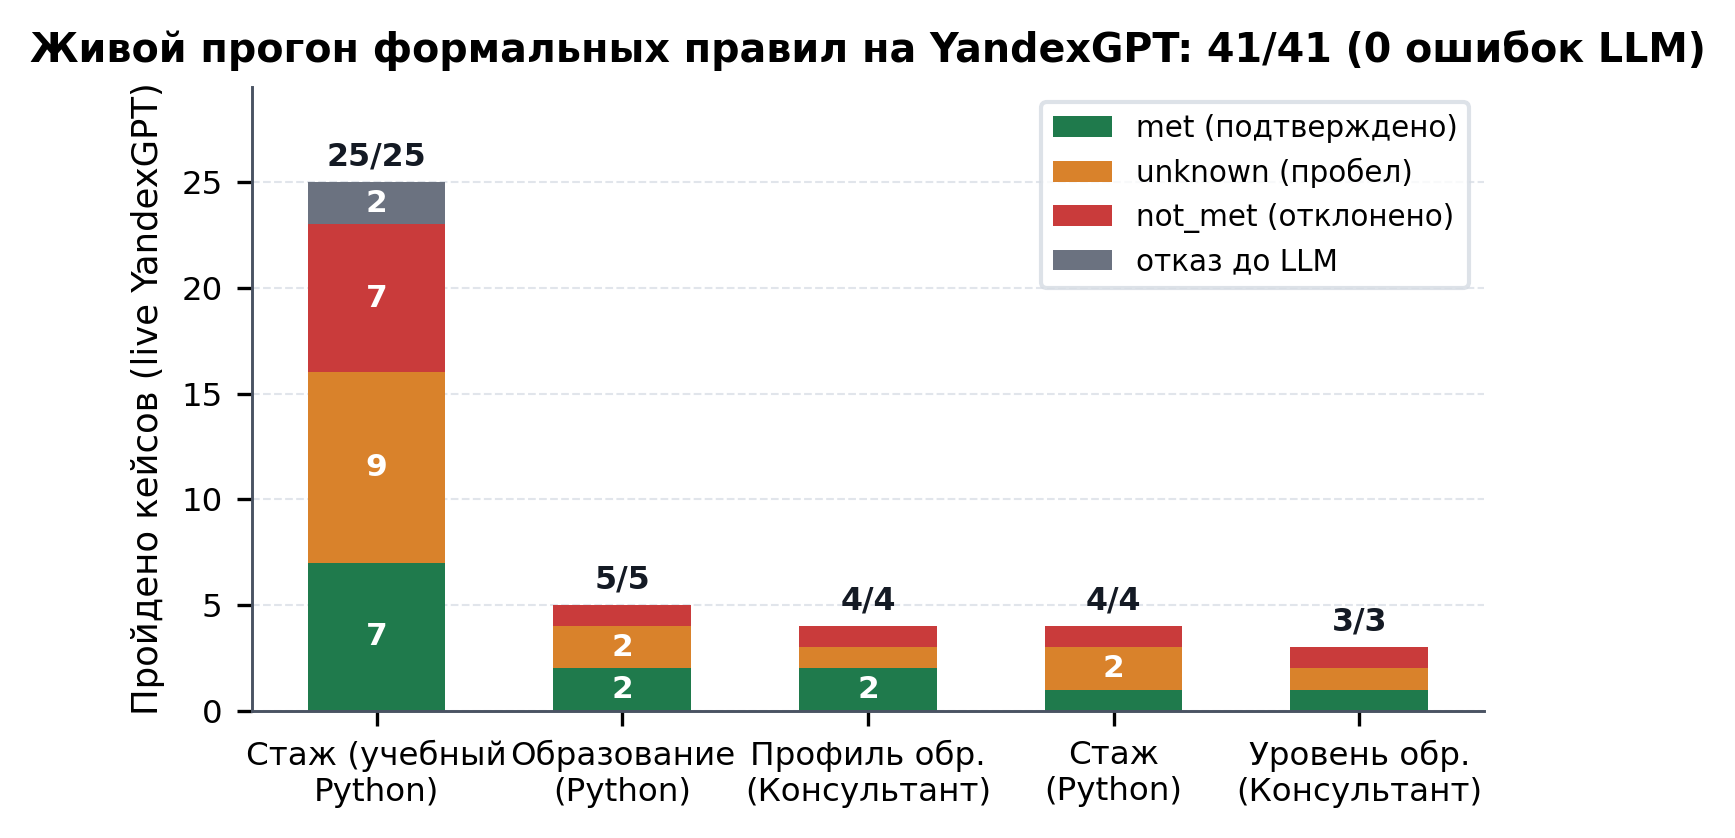
\includegraphics[width=\columnwidth]{figures/assessment_cases.png}
\caption{Разбивка 41 формального кейса живого прогона на YandexGPT
(\code{requirement-cases-live-pr15-fixes-2026-11-20.json}, \code{assessment-2.0.2},
\code{assess-v4}): 41/41 пройдено, 0 ошибок модели.}
\label{fig:assess}
\end{figure}

Контрольный пакет формальных правил проверен как в контролируемом режиме (код без сети), так и
в живом прогоне на \code{yandexgpt/latest} (\code{requirement-cases-live-pr15-fixes-2026-11-20.json},
рис.~\ref{fig:assess}): пройдено \textbf{41 из 41 кейсов} при 0 ошибках модели (39 живых
вызовов LLM и 2 отказа валидации до модели; 15 \code{unknown}, 13 \code{met}, 11 \code{not\_met},
2 \code{processing\_error}; 25 вердиктов подтверждены 1--4 верифицированными цитатами). Важное
уточнение границ: этот живой замер выполнен на версии \code{assessment-2.0.2} (проверка целевого
формального правила без записи в БД); уточнения версий \code{2.0.3}--\code{2.0.4} покрыты
автоматическими регрессионными тестами \code{pytest} без повторного живого вызова YandexGPT.

\subsection{Гайд телефонного интервью (\code{guide-v2})}

Модуль \code{app/interview/} формирует вопросы строго по открытым пробелам конкретной оценки:
код (\code{assemble\_gaps}, бюджет 6 вопросов, до 3 единиц на пробел) собирает список
недостающих сведений, а LLM (\code{guide-v2}) формулирует короткие вопросы и ориентиры ответа,
\textbf{не получая текста резюме} (только заголовки пробелов, \code{acceptance} и известные цитаты)
с проверкой ключей динамической схемой Pydantic. Ответы хранятся с ревизиями и оптимистической
блокировкой (\code{expected\_revision}), а подтверждение формального требования допускается
только по матрице оснований \code{\_CONFIRM\_BASES} (устные слова кандидата не заменяют диплом
или трудовую книжку).

\section{Поиск по опыту: BM25 против E5 + RRF}

Модуль \code{app/search/} решает задачу повторного поиска людей в кадровом архиве по
профессиональному опыту. Перед индексацией \code{text.py} отсекает архивный подвал («История
общения», «Отклик на вакансию»), сохраняет доменные токены (\code{25-ФЗ}, \code{1С},
\code{C++}, \code{Node.js}, \code{.NET}) и отфильтровывает фрагменты с прямым отрицанием
искомого навыка. Поддержаны две ветки ранжирования и их объединение через Reciprocal Rank
Fusion \citep{cormack2009rrf} с $k = 60$:
\begin{itemize}
  \item \textbf{Лексическая:} BM25 \citep{robertson2009bm25} с $k_1 = 1{,}2$, $b = 0{,}75$ и
    поддержкой обязательных точных терминов;
  \item \textbf{Векторная (опциональная):} локальная модель \code{intfloat/multilingual-e5-small}
    \citep{wang2024e5} (размерность 384, закреплённая ревизия, точное косинусное сходство в
    \code{pgvector}).
\end{itemize}

\begin{figure*}[t]
\centering
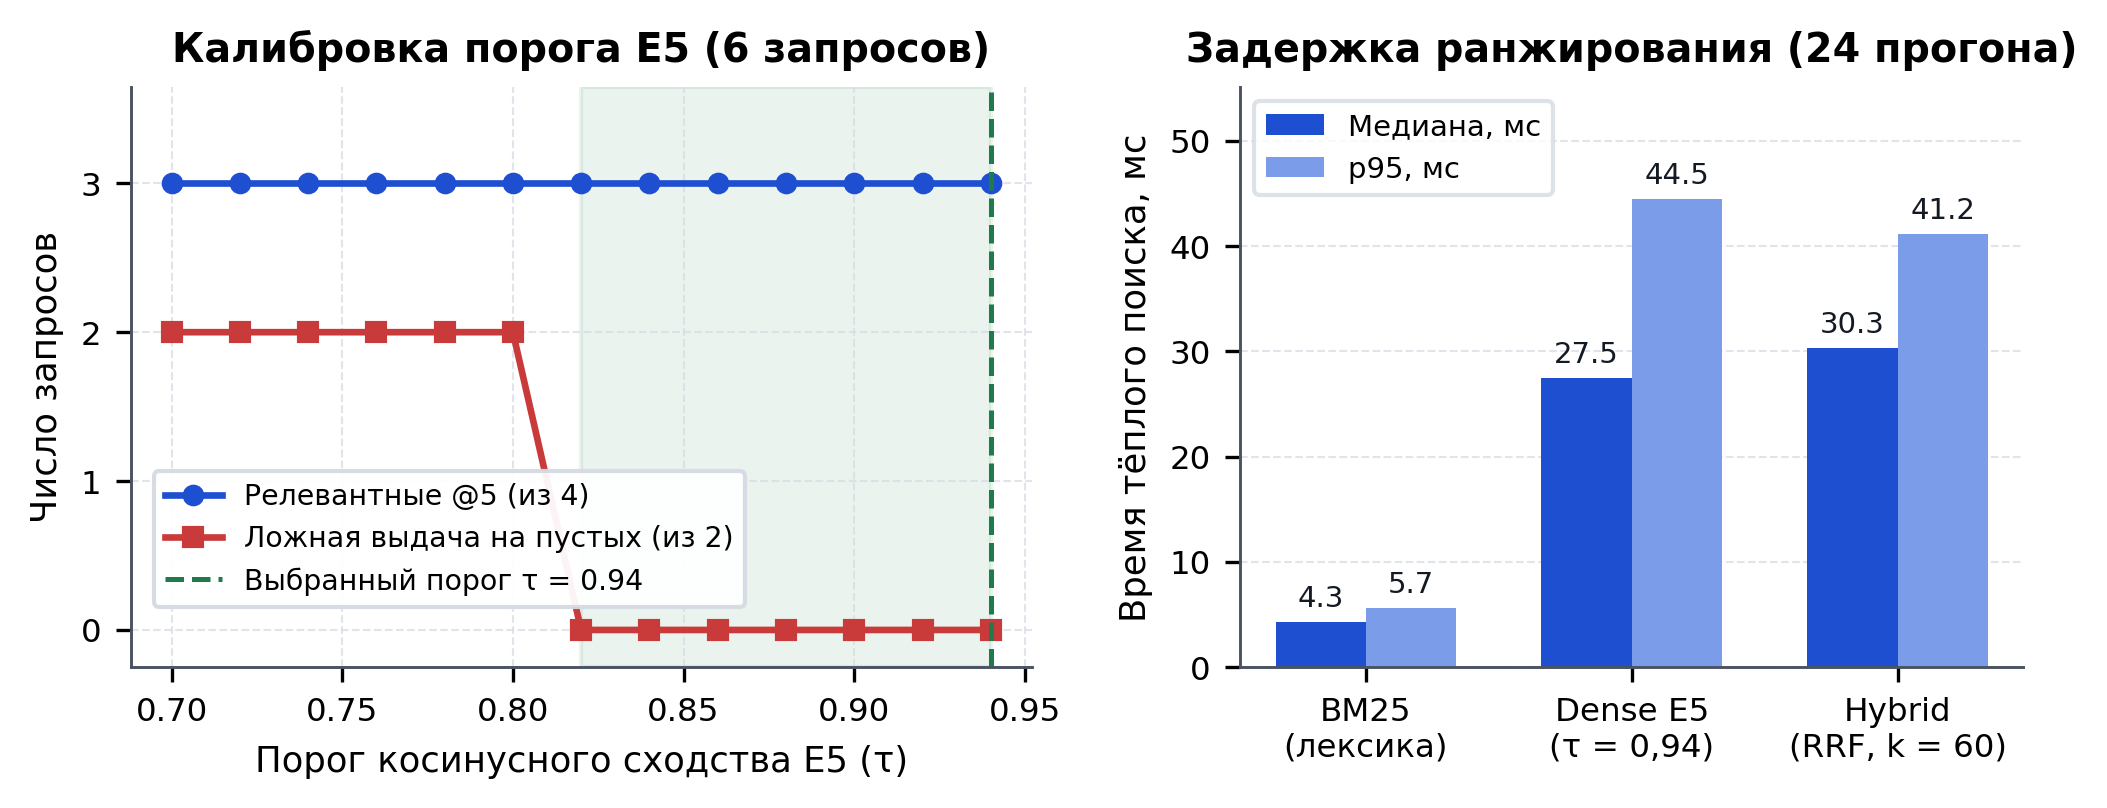
\includegraphics[width=0.92\textwidth]{figures/search_benchmark.png}
\caption{Результаты воспроизводимого бенчмарка поиска (\code{search-evaluation-v1.json}, 18
документов, 25 фрагментов). Слева: калибровка порога $\tau$ для E5 на 6 запросах (нулевая
ложная выдача достигается при $\tau \ge 0{,}82$, выбран строгий $\tau = 0{,}94$). Справа:
задержка тёплого ранжирования на 24 прогонах (без HTTP и БД).}
\label{fig:search}
\end{figure*}

\begin{table}[t]
\centering\footnotesize
\setlength{\tabcolsep}{3.5pt}
\begin{tabularx}{\columnwidth}{@{}Lrrrr@{}}
\toprule
Метод & Рел./пр. & Ложн. & Мед.,\,мс & p95,\,мс \\
\midrule
BM25 & 6 / 1 & 0 / 2 & \textbf{4,33} & \textbf{5,66} \\
Dense E5 ($\tau{=}0{,}94$) & 0 / 7 & 0 / 2 & 27,50 & 44,47 \\
Hybrid (RRF) & 6 / 1 & 0 / 2 & 30,32 & 41,17 \\
\bottomrule
\end{tabularx}
\caption{Контрольный замер поиска (\code{search-evaluation-v1.json}, 8 контрольных запросов,
24 замера времени, CPU PyTorch~2.14.1). Холодная загрузка модели E5 занимает 26,25\,с.}
\label{tab:search}
\end{table}

На закреплённом синтетическом наборе \code{search-01-synthetic-v1} (18 документов, 25 фрагментов,
6 калибровочных и 8 контрольных запросов, рис.~\ref{fig:search} и табл.~\ref{tab:search})
калибровка порога $\tau$ показала, что при $\tau \le 0{,}80$ модель E5 даёт ложную выдачу на
обоих внепредметных запросах (2/2). Выбор строгого порога $\tau = 0{,}94$ полностью обнулил
ложные срабатывания, но на контрольной выборке плотная ветка не вернула ни одного релевантного
кандидата (0/7), тогда как BM25 нашёл 6 из 7 релевантных (7/7 валидных UTF-16 цитат, 0/2
ложных), уступив лишь на одном перефразировании (\code{t-citizens}), и сработал в \textbf{6,4
раза быстрее} (4,33 против 27,50\,мс; без 26,25\,с холодной загрузки PyTorch).

На основании этого эксперимента (\code{hybrid\_meets\_local\_rule = false}) команда осознанно
оставила \code{HR\_SEARCH\_SEMANTIC\_ENABLED = false} в продовой конфигурации
\code{deploy/compose.yaml}, сохранив векторную ветку как включаемый флаг до накопления
рабочей разметки запросов кадровой службы.

\section{Отчётность, полнота данных и покрытие потребностей}

\subsection{Иммутабельные SHA-256 снимки и модель полноты}

Модуль годовой отчётности (\code{app/reporting/}) и адаптер управленческой картины
(\code{app/management/}) разделяют оперативную аналитику (\code{GET /api/v1/analytics/dashboard}
по живой БД) и официальный годовой доклад. Каждый выпуск годового доклада канонизируется и
сохраняется атомарно под ключом SHA-256 от содержимого (\code{store.py}): поздняя правка
исторического события не переписывает опубликованный документ, а порождает новый снимок.
Из того же снимка библиотека \code{xlsxwriter} (\code{excel.py}) строит многостраничную книгу
Excel с нативными диаграммами и листом методики.

Ключевое методологическое решение (\code{engine.py}) — четырёхзначная модель полноты каждой
ячейки: \code{complete}, \code{partial}, \code{unavailable}, \code{future}. В контрольном
прогоне волны~6 (\code{wave-6-report-demo.md}, 4 отклика, книга 18\,376 байт) октябрь 2026
получает по откликам \code{0 complete} (подтверждённый ноль при заявленном покрытии), а по
разговорам — \code{null unavailable} (источник не покрыт, цифра не приравнивается к нулю).
После внесения поздней поправки \code{rep-9004} выпущен второй снимок (разговоры ноября
$1 \to 2$ \code{partial}), при этом первый снимок при перечитывании остался побайтово неизменным.

\subsection{Независимое покрытие потребностей (алгоритм Куна)}

В модуле плановых срезов (\code{app/management/plans.py}, \code{max-bipartite-matching/augmenting-paths-v1})
решена типовая ошибка кадрового планирования — двойной учёт одного кандидата на несколько
открытых позиций. Пусть $S$ — множество открытых слотов вакансий, $P$ — множество
подтверждённых людей с доступным контактом, а ребро $(s, p) \in E$ означает подтверждённую
пригодность человека $p$ к слоту $s$. Вместо жадного подсчёта по каждой вакансии отдельно код
вычисляет размер максимального паросочетания в двудольном графе $G = (S, P, E)$ методом
увеличивающих путей Куна (\code{maximum\_matching}), возвращая точную верхнюю границу
одновременно закрываемых мест \code{independent\_total} и список предупреждений о концентрации
\code{concentrated} для всех людей степени $\deg(p) > 1$.

\section{Контроль SLA и композиция единого окна}

Для устранения «чёрной дыры» после передачи кандидата в департамент в \code{app/api/handoff.py}
и \code{app/db/calendar.py} реализован контроль срока в \textbf{10 рабочих дней} по
производственному календарю РФ (напоминание с 7-го рабочего дня), история переносов срока
(\code{HandoffDeadlineExtension}), версионные отзывы подразделения и оптимистическая блокировка
этапов \code{expected\_seq}.

В рамках этапа~2 в \code{c87cbd6} дополнительно реализован серверный механизм единого окна
ожиданий (\code{app/api/interaction.py}, \code{services/hiring/hiring/interaction\_window.py},
миграция \code{0014}): композиция обращений кандидата (Hiring) и передач в департаменты (Legacy)
с узкими SQL-выборками, подписанными HMAC-SHA256 курсорами пагинации, сущностью
\code{FeedbackReview}, ссылкой \code{Q-ref} и явной деградацией \code{complete}/\code{partial}/
\code{unavailable} при отказе одного из источников. В локальном ASGI-прогоне
(\code{docs/reports/interaction-window.md}) подтверждено 4/4 сценария за 3,11\,с (8 чтений,
максимум 39,4\,мс, максимум 7\,727 байт ответа при бюджете 3\,с и 256\,КиБ). На текущем стенде
единое окно намеренно выключено по умолчанию (\code{INTERACTION\_ENABLED = false}, выделено в
профиль \code{deploy/compose.interaction.yaml}) до подключения отдельного UI.

\section{Сводка проверок и ограничения}

В репозитории \code{c87cbd6} содержится \textbf{109 тестовых файлов} (\code{66} в корневом
\code{tests/} и \code{43} в \code{services/*/tests/}). В табл.~\ref{tab:eval} сведены
ключевые зафиксированные в \code{docs/reports/} проверки с точным указанием версии кода и
границ применимости (результаты разных коммитов не смешиваются).

\begin{table}[t]
\centering\small
\begin{tabularx}{\columnwidth}{@{}lLr@{}}
\toprule
Проверка & Область и условия & Итог \\
\midrule
\code{pgvector-full} & \code{6c5f9ba}, PG 16.15 + pgvector, миграции & 570 / 570 \\
\code{requirements-03} & \code{279c4609}, PG + pgvector, 1 skip (Node) & 831 pass \\
\code{wave-4c} & Полный набор ядра \code{legacy}, 0 skip & 898 / 898 \\
Live YandexGPT & \code{assessment-2.0.2}, целевое правило & 41 / 41 \\
Реестр публикаций & Реальный архив, 287 DOCX консультанта & 100\,\% детерм. \\
Бенчмарк поиска & 18 док., BM25 vs E5 (in-memory) & 6/7 (4,3\,мс) \\
Единое окно & ASGI/SQLite, деградация + отзыв прав & 4 / 4 (39,4\,мс) \\
Волны 1--6 (сервисы) & Сквозные HTTP-прогоны 8 сервисов & pass \\
\bottomrule
\end{tabularx}
\caption{Сводка верифицированных проверок по протоколам в \code{docs/reports/} и
\code{docs/modules/search-evaluation-v1.json}.}
\label{tab:eval}
\end{table}

\textbf{Честные ограничения текущей версии:}
\begin{itemize}
  \item Живой прогон на YandexGPT (41/41) зафиксирован на \code{assessment-2.0.2}; правила
    \code{2.0.3}--\code{2.0.4} подтверждены регрессионными тестами \code{pytest} на мок-клиенте,
    но не перезапускались на живой модели.
  \item Бенчмарк поиска выполнен на 18 синтетических документах без PostgreSQL/HTTP; качество
    поиска на рабочем корпусе требует разметки кадровой службы.
  \item Все шесть профилей из \code{all\_six} имеют статус \code{draft}; на учебном стенде
    утверждаются только их учебные копии.
  \item Пять из девяти сервисов этапа~1 используют SQLite и учебную авторизацию
    (\code{fixture}/\code{demo}); для промышленной эксплуатации требуются единая
    аутентификация (SSO), миграция на PostgreSQL и автоматический обмен событиями
    \code{Hiring}~$\to$~\code{Workforce}.
  \item В интерфейсе стенда модули \code{mobility}, \code{recognition} (раздел «Забота»),
    психометрика, OCR сканов и официальный конкурсный кадровый резерв честно помечены как
    следующий этап.
\end{itemize}

\section{Заключение}

Опыт разработки «Кадрового ассистента» показывает, что в задачах государственного и
муниципального управления наибольший эффект даёт не «универсальный ИИ-оценщик», а строгий
гибридный конвейер: обезличивание текста до вызова модели, детерминированный допуск по реестру
публикаций, верификация каждой цитаты кодом, интервальная арифметика стажа, честный отказ от
избыточных ML-компонентов при отсутствии измеримого выигрыша и математически корректная
отчётность. Все исходные коды, 109 тестовых файлов, JSON-протоколы замеров и скрипт генерации
графиков статьи (\code{docs/paper/build\_figures.py}) находятся в репозитории и полностью
воспроизводимы.

{\small
\bibliographystyle{plainnat}
\begin{thebibliography}{9}
\setlength{\itemsep}{2pt}
\expandafter\ifx\csname url\endcsname\relax\def\url#1{\texttt{#1}}\fi

\bibitem[Cormack et~al.(2009)]{cormack2009rrf}
Gordon~V. Cormack, Charles L.~A. Clarke, and Stefan Buettcher. 2009. Reciprocal rank fusion
outperforms Condorcet and individual rank learning methods. In \emph{Proceedings of SIGIR 2009},
pages 758--759.

\bibitem[Gao et~al.(2023)]{gao2023alce}
Tianyu Gao, Howard Yen, Jiatong Yu, and Danqi Chen. 2023. Enabling large language models to
generate text with citations (ALCE). In \emph{Proceedings of EMNLP 2023}, pages 6465--6488.

\bibitem[Korobov(2015)]{korobov2015morphological}
Mikhail Korobov. 2015. Morphological analyzer and generator for Russian and Ukrainian languages.
In \emph{Analysis of Images, Social Networks and Texts (AIST 2015)}, pages 320--332.

\bibitem[Robertson and Zaragoza(2009)]{robertson2009bm25}
Stephen Robertson and Hugo Zaragoza. 2009. The probabilistic relevance framework: BM25 and beyond.
\emph{Foundations and Trends in Information Retrieval}, 3(4):333--389.

\bibitem[Wang et~al.(2024)]{wang2024e5}
Liang Wang, Nan Yang, Xiaolong Huang, Linjun Yang, Rangan Majumder, and Furu Wei. 2024.
Multilingual E5 text embeddings: A technical report. \emph{arXiv preprint arXiv:2402.05672}.

\end{thebibliography}
}

\end{document}
